% hm-02-narriden.tex
\documentclass[xcolor=dvipsnames]{beamer}

\usepackage{graphicx}
% \usepackage{wrapfig}
% \usepackage{colortbl}
\usepackage{alltt}
% \definecolor{myblue}{rgb}{0.8,0.85,1}

\mode<presentation>
{
  \usetheme{Warsaw}
  \setbeamercovered{transparent}
}
% \usecolortheme[named=OliveGreen]{structure}
\setbeamertemplate{navigation symbols}{} 
\setbeamertemplate{blocks}[rounded][shadow=true] 

\newif\ifBCITCourse
\BCITCoursetrue
\BCITCoursefalse
\newif\ifWhichCourse
\WhichCoursetrue
% \WhichCoursefalse
\ifBCITCourse
\ifWhichCourse
\newcommand{\CourseName}{Statistics for Food Technology}
\newcommand{\CourseNumber}{MATH 1441}
\newcommand{\CourseInst}{BCIT}
\else
\newcommand{\CourseName}{Calculus for Geomatics}
\newcommand{\CourseNumber}{MATH 1511}
\newcommand{\CourseInst}{BCIT}
\fi
\else
\newcommand{\CourseName}{Philosophy and Literature}
\newcommand{\CourseNumber}{PHIL 375}
\newcommand{\CourseInst}{UBC}
\fi

\title{Narrative Self-Constitution}
\subtitle{{\CourseNumber}, {\CourseInst}}

\author{\CourseName}

\date{October 3, 2017}

% \begin{frame}
%   \frametitle{iClicker Question One}
% Choose from the following options. This item will be graded.
% \begin{block}{iClicker Question}
  
% \end{block}
% \begin{description}
% \item[A\hspace{.2in}$\blacktriangleright$] 
% \item[B\hspace{.2in}$\blacktriangleright$] 
% \item[C\hspace{.2in}$\blacktriangleright$] 
% \item[D\hspace{.2in}$\blacktriangleright$] 
% \item[E\hspace{.2in}$\blacktriangleright$] 
% \item[F\hspace{.2in}$\blacktriangleright$] 
% \end{description}
% \end{frame}

% \begin{figure}[h]
% \includegraphics[scale=.3]{./extrema1.png}
% \end{figure}

\begin{document}

\begin{frame}
  \titlepage
\end{frame}

% \begin{frame}
%   \frametitle{Structuralism Table}
% \begin{figure}[h]
% 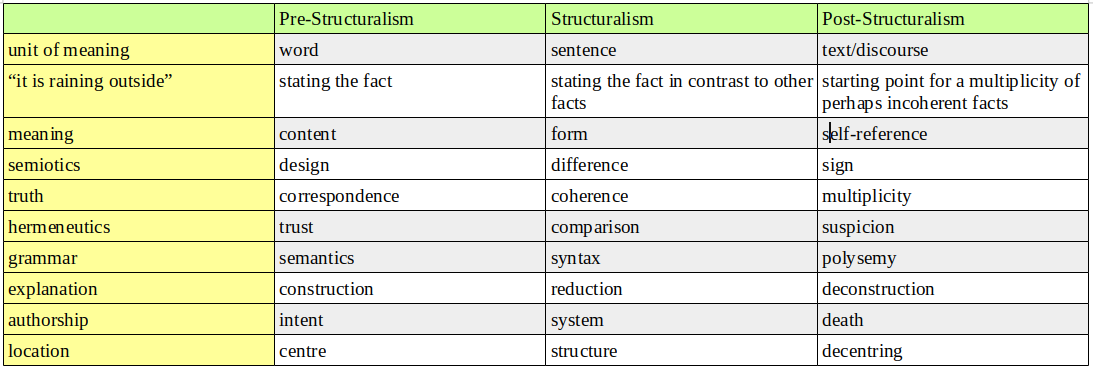
\includegraphics[scale=.3]{./structable.png}
% \end{figure}
% \end{frame}

% \begin{frame}
%   \frametitle{iClicker Question}
% Choose from the following options. This item will not be graded.
% \begin{block}{iClicker Question}
% Who argued that death is not an evil because it can only do harm to
% someone who no longer exists?
% \end{block}
% \begin{description}
% \item[A\hspace{.2in}$\blacktriangleright$] Gareth Evans
% \item[B\hspace{.2in}$\blacktriangleright$] Marcus Aurelius
% \item[C\hspace{.2in}$\blacktriangleright$] Epicurus
% \item[D\hspace{.2in}$\blacktriangleright$] Jeff McMahan
% \end{description}
% \end{frame}

% \begin{frame}
%   \frametitle{iClicker Question}
% Choose from the following options. This item will be graded.
% \begin{block}{iClicker Question}
% Which two movies are compared in Richard Kearney's article with
% respect to their use of narrative?
% \end{block}
% \begin{description}
% \item[A\hspace{.2in}$\blacktriangleright$] Milo{\^s} Forman's \emph{Amadeus} and Philip Kaufman's \emph{The Unbearable Lightness of Being}
% \item[B\hspace{.2in}$\blacktriangleright$] Robert Zemecki's \emph{Forrest Gump} and James Cameron's \emph{Titanic}
% \item[C\hspace{.2in}$\blacktriangleright$] Steven Spielberg's \emph{Schindler's List} and Claude Lanzmann's \emph{Shoah}
% \item[D\hspace{.2in}$\blacktriangleright$] The Wachowski's \emph{The Matrix} and Christopher Nolan's \emph{Inception}
% \end{description}
% \end{frame}

% \begin{frame}
%   \frametitle{iClicker Question}
% Choose from the following options. This item will be graded.
% \begin{block}{iClicker Question}
% For which philosopher's account of personal identity does Marya
% Schechtman point out that it rests on consciousness rather than, as
% usually assumed, memory?
% \end{block}
% \begin{description}
% \item[A\hspace{.2in}$\blacktriangleright$] John Locke
% \item[B\hspace{.2in}$\blacktriangleright$] David Hume
% \item[C\hspace{.2in}$\blacktriangleright$] J.S. Mill
% \item[D\hspace{.2in}$\blacktriangleright$] Immanuel Kant
% \end{description}
% \end{frame}

% \begin{frame}
%   \frametitle{iClicker Question}
% Choose from the following options. This item will be graded.
% \begin{block}{iClicker Question}
% Which of these are not part of a Schechtman illustration in her paper?
% \end{block}
% \begin{description}
% \item[A\hspace{.2in}$\blacktriangleright$] the fat lady in the picture
% \item[B\hspace{.2in}$\blacktriangleright$] the sing-song of old man kangaroo
% \item[C\hspace{.2in}$\blacktriangleright$] the man who thought he was Napoleon
% \item[D\hspace{.2in}$\blacktriangleright$] Dr. Bernheim's umbrella
% \end{description}
% \end{frame}

% \begin{frame}
%   \frametitle{iClicker Question}
% Choose from the following options. This item will be graded.
% \begin{block}{iClicker Question}
% What is the cornerstone of existentialism?
% \end{block}
% \begin{description}
% \item[A\hspace{.2in}$\blacktriangleright$] man's existence is more firmly established than God's existence
% \item[B\hspace{.2in}$\blacktriangleright$] existence precedes essence
% \item[C\hspace{.2in}$\blacktriangleright$] man is not free but bound to his existence
% \item[D\hspace{.2in}$\blacktriangleright$] everything is morally permissible
% \end{description}
% \end{frame}

% \begin{frame}
%   \frametitle{iClicker Question}
% Choose from the following options. This item will be graded.
% \begin{block}{iClicker Question}
% Which of these are not part of a Sartre illustration in his paper?
% \end{block}
% \begin{description}
% \item[A\hspace{.2in}$\blacktriangleright$] joining the resistance or staying with one's mother
% \item[B\hspace{.2in}$\blacktriangleright$] the picture of Dorian Gray
% \item[C\hspace{.2in}$\blacktriangleright$] a man who becomes a Jesuit after many setbacks in life
% \item[D\hspace{.2in}$\blacktriangleright$] joining a Christian or a Communist trade union
% \end{description}
% \end{frame}

% \begin{frame}
%   \frametitle{iClicker Question}
% Choose from the following options. This item will be graded.
% \begin{block}{iClicker Question}
% Which one of these is a core moral dilemma in Charles Taylor's essay
% ``What Is Human Agency?''?
% \end{block}
% \begin{description}
% \item[A\hspace{.2in}$\blacktriangleright$] legalizing abortion vs valuing human life
% \item[B\hspace{.2in}$\blacktriangleright$] eating organic local food vs giving to charity
% \item[C\hspace{.2in}$\blacktriangleright$] persisting in an academic job vs moving to Nepal
% \item[D\hspace{.2in}$\blacktriangleright$] keeping one healthy person alive vs having five sick patients die
% \end{description}
% \end{frame}

% \begin{frame}
%   \frametitle{iClicker Question}
% Choose from the following options. This item will be graded.
% \begin{block}{iClicker Question}
% Which of these contrast pairs is not a distinction found in Charles
% Taylor's paper?
% \end{block}
% \begin{description}
% \item[A\hspace{.2in}$\blacktriangleright$] internalist and externalist evaluation
% \item[B\hspace{.2in}$\blacktriangleright$] first and second order desires
% \item[C\hspace{.2in}$\blacktriangleright$] qualitative and quantitative evaluation
% \item[D\hspace{.2in}$\blacktriangleright$] weak and strong evaluation
% \end{description}
% \end{frame}

% \begin{frame}
%   \frametitle{iClicker Question}
% Choose from the following options. This item will be graded.
% \begin{block}{iClicker Question}
% On the Non-Reductionist view, according to Derek Parfit in the reading for today,
% \end{block}
% \begin{description}
% \item[A\hspace{.2in}$\blacktriangleright$] moral choices cannot be reduced to calculations about consequences
% \item[B\hspace{.2in}$\blacktriangleright$] a person is a separately existing entity, distinct from brain, body, and experience
% \item[C\hspace{.2in}$\blacktriangleright$] moral questions cannot be reduced to scientific questions
% \item[D\hspace{.2in}$\blacktriangleright$] Buddha's message and the Judaeo-Christian message cannot be reduced to each other
% \end{description}
% \end{frame}

% \begin{frame}
%   \frametitle{iClicker Question}
% Choose from the following options. This item will be graded.
% \begin{block}{iClicker Question}
% What is Hume's comparison for the soul?
% \end{block}
% \begin{description}
% \item[A\hspace{.2in}$\blacktriangleright$] a republic or commonwealth, in which the several members are united by the reciprocal ties of government and subordination
% \item[B\hspace{.2in}$\blacktriangleright$] a prisoner of war, always treated with a respect suitable to his condition
% \item[C\hspace{.2in}$\blacktriangleright$] a commander in charge of a ship, communicating with the several parts of a vessel
% \item[D\hspace{.2in}$\blacktriangleright$] a soup, in which the ingredients are now united though they were once asunder
% \end{description}
% \end{frame}

% \begin{frame}
%   \frametitle{iClicker Question}
% Choose from the following options. This item will be graded.
% \begin{block}{iClicker Question}
% What game did Hume play to distract himself from the depressing
% conclusions of his philosophical thought?
% \end{block}
% \begin{description}
% \item[A\hspace{.2in}$\blacktriangleright$] chess
% \item[B\hspace{.2in}$\blacktriangleright$] bridge
% \item[C\hspace{.2in}$\blacktriangleright$] backgammon
% \item[D\hspace{.2in}$\blacktriangleright$] tennis
% \end{description}
% \end{frame}

\begin{frame}
  \frametitle{Two Claims}
  \begin{description}
  \item[psychological thesis] this is a descriptive, empirical claim
    about the nature of ordinary human experience, where a lack of
    narrativity is pathological with respect to how ordinary that
    experience is
  \item[ethical thesis] this is a normative, ethical claim that a
    narrative outlook is essential to a well-lived life, to true or
    full personhood
  \end{description}
\end{frame}

\begin{frame}
  \frametitle{Combinations of the Two Claims}
  \begin{tabular}{|l|l|l|}\hline
    \hspace{.5in}               & \hspace{.5in}        & \hspace{.5in}  \\
                                & psychological thesis & ethical thesis \\
    \hspace{.5in}               & \hspace{.5in}        & \hspace{.5in}  \\ \hline
    \hspace{.5in}               & \hspace{.5in}        & \hspace{.5in} \\
    Sartre/Stoics               & yes                  & no             \\
    \hspace{.5in}               & \hspace{.5in}        & \hspace{.5in}  \\ \hline
    \hspace{.5in}               & \hspace{.5in}        & \hspace{.5in} \\
    Plutarch                    & no                   & yes            \\ 
    \hspace{.5in}               & \hspace{.5in}        & \hspace{.5in}  \\ \hline
    \hspace{.5in}               & \hspace{.5in}        & \hspace{.5in} \\
    Schechtman/Taylor/MacIntyre & yes                  & yes            \\ 
    \hspace{.5in}               & \hspace{.5in}        & \hspace{.5in}  \\ \hline
    \hspace{.5in}               & \hspace{.5in}        & \hspace{.5in} \\
    Strawson                    & no                   & no             \\ 
    \hspace{.5in}               & \hspace{.5in}        & \hspace{.5in}  \\ \hline
  \end{tabular}
\end{frame}

\begin{frame}
  \frametitle{Relevant Questions}
  \begin{itemize}
  \item What are persistence conditions?
  \item What is the difference between a human being and a subjectively
    experienced self?
  \item What is true about these intuitions: the chilling, empty
    deficiency of the Episodic life versus the macerated, clogged,
    excessively self-concerned, inauthentically second-order qualities
    of the Diachronic life?
  \item Does it make a difference to be explicitly or implicitly
    narrativizing?
  \end{itemize}
\end{frame}

\begin{frame}
  \frametitle{The Episodic Life}
  \begin{block}{Against Narrativity, page 433}
    I have absolutely no sense of my life as a narrative with form, or
    indeed as a narrative without form. Absolutely none. Nor do I have
    any great or special interest in my past. Nor do I have a great
    deal of concern for my future.
  \end{block}
\end{frame}

\begin{frame}
  \frametitle{More Relevant Questions}
  \begin{itemize}
  \item How is it that the from-the-inside quality of a memory can be
    detached from any sense that one is the subject of the remembered
    experience (434)?
  \item Does Strawson give a satisfying answer to what it is to have
    or be a self? Is there an abolition of selfhood lurking in the
    background? Who am I, and if so, how many? (Richard David Precht)
    See also \emph{The Ego Tunnel} by Thomas Metzinger or \emph{The
      Architecture of the Mind} by Peter Carruthers. What are the
    metaphysics of selfhood?
  \item How do you assess Strawson's argument that the ethical
    narrativity claim is associated with self-importance, religion,
    and narcissism (436f)?
  \end{itemize}
\end{frame}

\begin{frame}
  \frametitle{More Relevant Questions}
  \begin{itemize}
  \item Does the making coffee narrative scale up to larger narratives
    and propagate to higher levels; or is Strawson correct to call the
    narrativity claim about short-term plans trivial?
  \item Has Strawson addressed the problem that narrativists have with
    an invasive scientific anthopology? (See footnote 27.)
  \item How can a narrative be defined stringently? Note Strawson's
    emphasis on developmental, temporal unity and coherence.
  \item What does a personal relationship with an Episodic look like?
  \end{itemize}
\end{frame}

\begin{frame}
  \frametitle{Conditions of Narrativity}
  \begin{description}
  \item[diachronicity] I identify myself (the one who is the receiver
    of my subjective experiences) with the human being that I was in
    the past and that I will be in the future
  \item[form-finding] I seek for coherence, unity, and pattern in the
    temporal sequence events in my life
  \item[story-telling] I think of my life in recognizable literary
    genres
  \item[revision] I distort facts about my life so that they fit the
    kind of story that I want to tell about myself (444)
  \end{description}
\end{frame}

\begin{frame}
  \frametitle{Strawson's Shift}
  There is a marked shift on page 447 to a negative evaluation of
  narrativity. There appears to be some inconsistency between the
  pre-447 Strawson and the post-447 Strawson.
\end{frame}

\begin{frame}
  \frametitle{Lanzmann versus Spielberg}
  Compare the following two film previews.
  \begin{alltt}
    https://www.youtube.com/watch?v=VXsgUnLG4CY
  \end{alltt}
  \begin{alltt}
    https://www.youtube.com/watch?v=JdRGC-w9syA
  \end{alltt}
\end{frame}

\begin{frame}
  \frametitle{The Four Features}
  Sentient beings and persons are distinguished by
  \begin{itemize}
  \item moral agency
  \item compensation
  \item self-interested concern
  \item survival
  \end{itemize}
  Individuals constitute themselves as persons by coming to think of
  themselves as persisting subjects who have had experience in the
  past and will continue to have experience in the future.
\end{frame}

\begin{frame}
  \frametitle{Constraints}
  \begin{description}
  \item[Articulation] Form and logic of a conventional, linear
    narrative. Constituents (characters, events) do not have a meaning
    on their own. Meaning comes from the configuration, from the plot.
    Time-slices are not fully intelligible. 
  \item[Reality] Self-constitution requires both an internal life and
    a proper connection to the social world. Self-conception must be
    in sync with that of others.
  \end{description}
  Mitigation of the ``no personhood without narrative'' claim: (i)
  other forms of existence are valuable; (ii) there is a wide
  diversity of qualifying narratives.
\end{frame}

\begin{frame}
  \frametitle{Parfit's Satori-Like Dissolution of the Self}
  Parfit concludes from the superficiality of psychological continuity
  that the self is a fiction. MS claims, however, that a Parfitian
  live-for-the-moment, sever-the-bonds-with-the-past-and-the-future
  life produces individuals who
  \begin{itemize}
  \item don't make plans
  \item don't engage in long-term commitments
  \item don't take responsibility for the past, and, in any case,
  \item don't embrace the concept of personhood
  \end{itemize}
  MS and DP only disagree on whether personhood is achievable without superficiality.
\end{frame}

\begin{frame}
  \frametitle{Marxist Concerns}
  A possible Marxist critique: the narrative self-constitution view is
  an insistence on conformity to the worldview of a dominant group. In
  response, Schechtman points out how much similarity there is between
  a revolutionary and a reactionary narrative compared to the contrast
  between a revolutionary narrative and the incoherence of a psychotic.
\end{frame}

\begin{frame}
  \frametitle{John Locke's Account of Personal Identity}
  Sameness of consciousness, not sameness of substance (Kafka's
  \emph{Metamorphosis}). The problem with a pure memory account of
  personal identity is that memories are by definition remembered,
  while consciousness can be affected more globally and partly
  subconsciously. Example: financial security.
\end{frame}

\begin{frame}
  \frametitle{Confabulation and Self-Blindness}
  Schechtman claims that to the extent to which we confabulate and
  deceive ourselves, our personhood is compromised. Umbrella episode
  with Dr.\ Bernheim. Heidegger/Habermas debate: does mysticism and
  ineffability enhance or reduce personhood?

  \bigskip

  Loss of personhood can also originate in not inhabiting the same
  world as one's fellows. MS puts much greater emphasis here on
  coherence of facts rather than coherence of interpretation (what
  about the first secular atheist, the psychopath, or the
  depressive?). 
\end{frame}

\begin{frame}
  \frametitle{Polyjuice Potion}
  Schechtman also claims that the narrative self-constitution view can
  mediate between two opposing views on continuity, the bodily vs the
  psychological continuity view. While the narrative self-constitution
  view is broadly supportive of the psychological view, it also
  underlines that the congress of body and person is not accidental.
\end{frame}

\begin{frame}
  \frametitle{I Have No Future}
  Epicurus' argument that death does no harm.
  \begin{enumerate}
  \item ``Look back at time {\ldots} our birth. In this way nature
    holds before our eyes the mirror of our future after death. Is
    this so grim, so gloomy?'' (Lucretius)
  \item ``Death {\ldots} the most awful of evils, is nothing to us,
    seeing that, when we are, death is not come, and, when death is
    come, we are not.'' (Letter to Menoeceus)
  \end{enumerate}
Strawson's argument is not psychological, but philosophical. 
\end{frame}

\begin{frame}
  \frametitle{Relevant Questions}
  \begin{itemize}
  \item What are things that can be taken away from us? (Our country,
    our human rights, {\ldots})
  \item Can retributive justice be squared with Strawson's NOF? Is
    Strawson's view consistent with his father's view that reactive
    attitudes are independent of metaphysical justifications or
    entitlements and cannot be in contradiction to determinism?
  \item Does Strawson succeed in explaining regret? See Thomas Nagel's
    paper ``Death'' (1970). Keats (24) and Tolstoy (82). 
  \item Is Strawson's account of depression believable, that the
    condition's referent is the present, not the future? Is it true
    that a depressed person's desire is the cessation of the present
    rather than the future?
  \end{itemize}
\end{frame}

\begin{frame}
  \frametitle{The Problem with Science}
  \begin{itemize}
  \item impersonal information
    \begin{itemize}
    \item disembodied (Cartesian, see page 36)
    \item digital vs analog
    \item quantitative vs qualitative
    \end{itemize}
  \item maintenance of civil society
  \item maintenance of historical memory (rather than annals)
  \end{itemize}
\end{frame}

\begin{frame}
  \frametitle{The Problem with Postmodernism}
  \begin{itemize}
  \item dissolution of \emph{les grands r{\'e}cits} (Lyotard)
  \item Baudrillard's ``mediatized culture of depthless simulation
    which abandons reference to historical reality'' (irreference)
  \item purveyors of prejudice
  \item fractured discursive practices about truth, identity, and the good
  \end{itemize}
\end{frame}

\begin{frame}
  \frametitle{Ricoeur's Synthesis of the Heterogeneous}
  Ethics, according to Ricoeur, is the link between happiness and
  virtue. A strictly scientific, de-narrativized view leads to
  collapse. Compare personal identity to an episode of romantic love.
  \begin{itemize}
  \item the other must have intrinsic value
  \item there must be a beginning, a middle, and an end
  \item there must be a poetic element, something to elevate it above
    the mundane
  \item a long-term romantic relationship integrates widely different
    tasks, such as family relations, business, child-rearing,
    sexuality, meaning $\longrightarrow$ synthesis of the heterogeneous
  \end{itemize}
\end{frame}

\begin{frame}
  \frametitle{The Economy of Romance}
  \begin{quote}
    {\ldots} after Katya broke up with him. He'd wanted to marry her
    and have a child. She needed someone more reliable, she said; he
    barely made enough to support a single frugal man skimpily and she
    also wanted to see what her value was on the social marketplace,
    as she put it {\ldots} (Stephen Dixon, Old Friends, 17)
  \end{quote}
  \begin{quote}
    The bourgeoisie {\ldots} has reduced the family relation to a mere
    money relation. (Communist Manifesto, cf.\ the Marxist concept of
    reification)
  \end{quote}
  See the work of Marina Adshade (entertainingly packaged in a TED
  Talk).
\end{frame}

\begin{frame}
  \frametitle{Aristotle's Ethics Sandbox}
  \begin{figure}[h]
    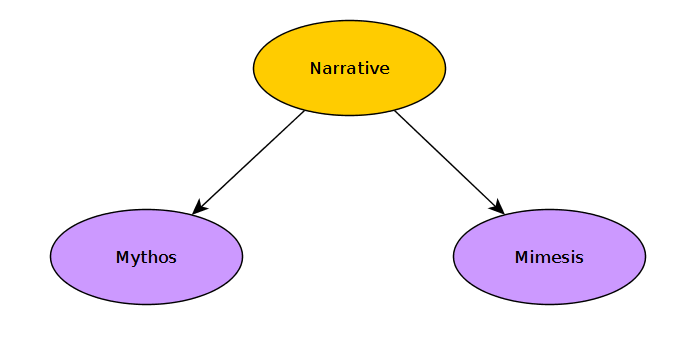
\includegraphics[scale=0.5]{./mythos.png}
  \end{figure}
\end{frame}

\begin{frame}
  \frametitle{Yes,  We Kant}
  Kearney claims that Kant's account of moral responsibility relies on
  narrative as much as Aristotle's. Hannah Arendt, a well-known
  Kantian, emphasizes the communicative nature of narrative where
  someone says something to someone about something $\longrightarrow$
  contrast to Roland Barthes with the death of the author. A Kantian
  view of moral responsibility needs a sensus communis, where I can
  imagine myself in the other and the other in myself. Ricoeur's
  \emph{moi} (self-same self) is transformed to \emph{soi}
  (self-for-others).
\end{frame}

\begin{frame}
  \frametitle{Kearney's Narrative Ethics View}
  \begin{block}{Richard Kearney, page 35}
    Narrative, understood from both and Aristotelian and Kantian
    perspective, can serve an indispensable function of ethical
    \emph{responsibility}. By recounting the story of one's life in
    response to the other's question---who are you?---the narrative
    self constitutes itself as a perduring identity over time, capable
    of sustaining commitments and pledges, that is, of keeping one's
    promises to the other.
  \end{block}
\end{frame}

\begin{frame}
  \frametitle{Fidelity}
  One cannot be faithful to one's word, unless one has a minimal
  grasp---through some form of narrative---of who one is (38).
  Ricoeur's two examples: the talking cure (psychoanalysis) and
  Biblical Israel. The hermeneutical circle (self-constitution) makes
  possible the co-existence of constancy and flexibility.
  Fundamentalism/nationalism: where the founding narrative is
  concealed.
\end{frame}

\begin{frame}
  \frametitle{Masters of Suspicion}
  Note here J{\"u}rgen Habermas' critique of ideology. A hermeneutic
  of affirmation/trust must be accompanied by a hermeneutics of
  suspicion. The three masters of suspicion:
  \begin{itemize}
  \item Nietzsche: narrative is the masking of will-to-power
  \item Marx: see Antonio Gramsci's theory of cultural hegemony
  \item Freud: narratives are often misleading signals of a rich
    subconscious life (amnesia of ontogenesis)
  \end{itemize}
\end{frame}

\begin{frame}
  \frametitle{The Historiography Debate}
  Ricoeur vs Hempel. Narrative vs generalizable laws and statistical
  data (the DN, deductive-nomological, and IS, inductive-statistical,
  model). Phronesis of singular narratives vs theoria of historical
  laws and facts.
\end{frame}

\begin{frame}
  \frametitle{Jacques Derrida I}
  \begin{quote}
    I understand that the question of the marriage vows was, this
    morning, considered interesting by some of you, the ``yes'' to the
    marriage, the performative ``yes'' -- ``I do'', ``I do''. This
    ``yes'' has to be repeated differently each time. If it's simply a
    record saying ``I do'' ``I do'' ``I do'' there is no fidelity. For
    this ``I do'' to be a renewed promise it has to be different each
    time, the same one and different. In order to follow the ``I do''
    today (before the priest), the ``idea'' of tomorrow should be the
    same and different {\ldots}
  \end{quote}
\end{frame}

\begin{frame}
  \frametitle{Jacques Derrida II}
  \begin{quote}
    {\ldots} They must follow one another and confirm themselves but,
    at the same time, be different. That's what the counter-signature
    is. Of course, even if I say to the same person ``I do'' tomorrow
    and after tomorrow, the fact that this ``I do'' is different, to
    some extent, means at the same time fidelity and betrayal. Indeed,
    it's a kind of perjury to say ``I do'' to someone. So that may be
    the paradox in the twin concepts of acoluthia and anacoluthon. You
    have to betray in order to be truthful. (Life After Theory, 10f)
  \end{quote}
\end{frame}

\begin{frame}
  \frametitle{Reproaches Against Existentialism}
  \begin{itemize}
  \item quietism (communists) intellectual contemplation leads to just
    another bourgeois worldview
  \item privileging the solitary over solidarity, forgetting the
    ``smile of the infant'' (Catholics)
  \item the seriousness of human affairs and moral responsibility (Christians)
  \end{itemize}
  JPS: They call us gloomy, when they say (dismal proverbs), ``charity
  begins at home''
\end{frame}

\begin{frame}
  \frametitle{Existence Precedes Essence}
  In the 18th century, the idea of the artisan-designer for human
  beings was sidelined, but the quest for a human essence remained.
  The paper knife.
  \begin{itemize}
  \item ``man surges up in the world and defines himself afterwards''
  \item man differs from a scientific object because he is nothing
    until he makes something of himself
  \item in choosing for himself he chooses for all men (Christian
    trade union, monogamy)
  \item man is condemned to be free
  \end{itemize}
\end{frame}

\begin{frame}
  \frametitle{Open Questions}
  \begin{itemize}
  \item How typical is the Free French example for a moral dilemma?
  \item Man fashions both the signs and their interpretation
    $\longrightarrow$ the importance of hermeneutics for ethics
    (Jesuit priest)
  \item Sartre's reliance on Kant (``one ought always to ask oneself
    what would happen if everyone did as one is doing,'' 292) and
    Descartes (``the starting point for truth is one's immediate sense
    of self'', 302)
  \item Contrast human nature with the human condition to understand
    what Sartre means by cowardice. ``Those who hide from total
    freedom, in a guise of solemnity or with deterministic excuses, I
    shall call cowards'' (308). The story of Carlos Flores and the
    subway accident.
  \item How appropriate is it to demand strict authenticity from
    humans? Don't we need an essence for authenticity, for ``being who
    we are''? Michel Foucault's criticism.
  \end{itemize}
\end{frame}

\begin{frame}
  \frametitle{Hermeneutic and Scientific Method}
  \begin{equation}
    \label{eq:paumatae}
    \begin{array}{rcl}
      \mbox{understanding} & \mbox{vs.} & \mbox{explaining} \\
      \mbox{narrative} & \mbox{vs.} & \mbox{model} \\
      \mbox{inter-textuality} & \mbox{vs.} & \mbox{experiment} \\
      \mbox{coherence} & \mbox{vs.} & \mbox{falsifiability} \\
      \mbox{hypostatic} & \mbox{vs.} & \mbox{hypothetical} \\
      \mbox{texts} & \mbox{vs.} & \mbox{nature} \\
      \mbox{integration} & \mbox{vs.} & \mbox{differentiation} \\
      \mbox{dialectic} & \mbox{vs.} & \mbox{monism} \\
    \end{array}\notag
  \end{equation}
\end{frame}

\begin{frame}
  \frametitle{The Hermeneutic Tradition}
\begin{figure}[h]
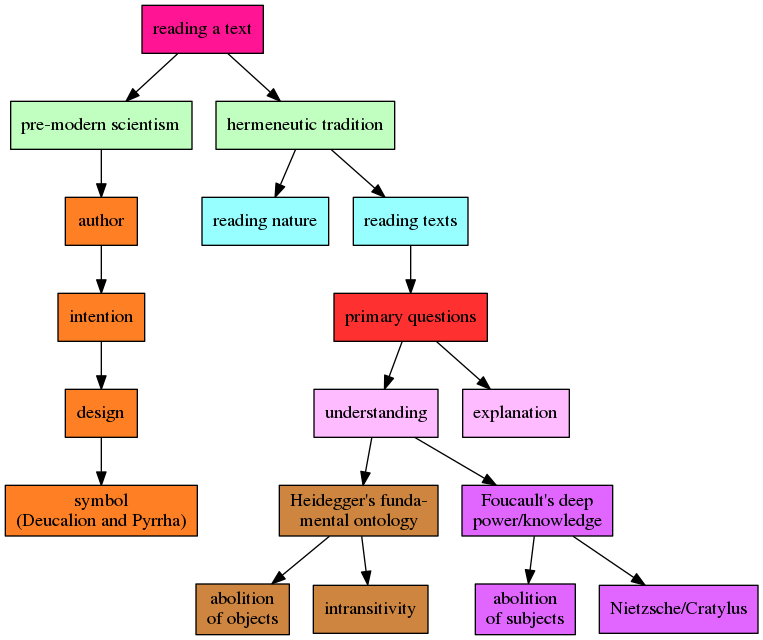
\includegraphics[scale=.32]{./subob.png}
\end{figure}
\end{frame}

\begin{frame}
  \frametitle{Structuralism}
\begin{figure}[h]
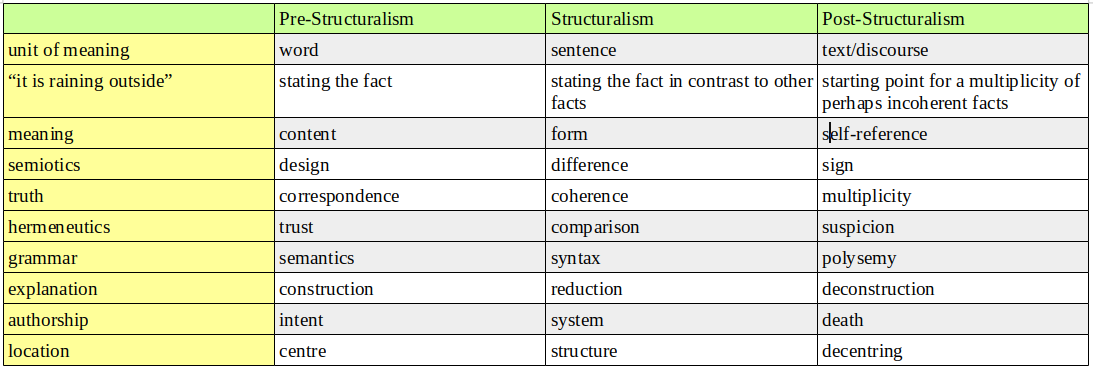
\includegraphics[scale=.3]{./structable.png}
\end{figure}
\end{frame}

\begin{frame}
  \frametitle{Frankfurt's Second-Order Desires}
  \begin{itemize}
  \item first-order and second-order desires
  \item qualitative and quantitative evaluation of desires
  \item weak and strong evaluation (the defining feature for strong
    evaluation is to have a qualitative distinction of the worth of
    the motivations)
  \end{itemize}
Utilitarianism fails on two counts:
\begin{enumerate}
\item weak evaluation is not reducible to calculation
\item moral evaluation is not reducible to weak evaluation
\end{enumerate}
\end{frame}

\begin{frame}
  \frametitle{Criteria for Distinction}
  \begin{description}
  \item[contingency] strong evaluation dilemmas cannot be resolved by appeal to contingencies
  \item[contrast] strong evaluation proceeds on the basis of
    contrasts (courage is meaningless without cowardice and vice
    versa)
  \end{description}
\end{frame}

\begin{frame}
  \frametitle{The Problem with Second-Order Desires}
\begin{itemize}
\item the practical vs the moral approach to raising children
\item consider a law that makes something morally repugnant
  (abortion, drug consumption, corruption, sex with children) more
  legal and less frequent $\longrightarrow$ would you assent to it?
\item are the moral notions at the basis of strong evaluation only
  a front to legitimize moral/social/economic pressure on others?
  (Mandeville)
\item the drug that allows you to eat cake and be healthy as well
  (deflated descriptions vs moral reality)
\item CT resolves this later by appealing to re-evaluation
\end{itemize}
\end{frame}

\begin{frame}
  \frametitle{J.S. Mill's Defence}
  Charles Taylor: ``honour, dignity, integrity are \emph{simply}
  other pleasurable states to which we give \emph{high-sounding}
  names'' (23). Why does reducibility in principle imply undue
  simplicity? Why is the ``simple weigher'' inferior to the
  ``strong evaluator''? Monism can be maintained even in the face
  of certain kinds of emergence.
  \begin{block}{Charles Taylor}
    thus the strong evaluator has articulacy and depth which the
    simple weigher lacks
  \end{block}
Really? Isn't it the monist who makes progress? Perhaps the monist
does not succeed with the reduction, but many productive (rather
than successful) scientific programs originate in a desire to
perform a reduction (alchemy). 
\end{frame}

\begin{frame}
  \frametitle{The Importance of Articulation}
  First-order choices are inarticulable. Second-order choices flow
  from the use of language and articulated coherence. Note the
  following analogy:
  \begin{itemize}
  \item Descartes' \textsc{je pense} solves an epistemological
    problem (skepticism); as a consequence, we perceive ourselves
    primarily and dominantly as thinking beings
  \item Taylor's \textsc{je parle} solves an ethical problem (what
    characterizes moral responsibility); as a consequence, we
    perceive ourselves primarily and dominantly as
    talking/interpreting/story-telling beings
  \end{itemize}
The story of my great-grandparents. 
\end{frame}

\begin{frame}
  \frametitle{Responsibility and Radical Choice}
  The problem with radical choice (Free French, Nepal) is that it
  solves the dilemma by rendering the force of the losing side
  inoperative (this is a problem that Bernard Williams has
  addressed with respect to utilitarianism and Kantian moral
  theory in articles such as ``Consequentialism and Integrity''
  and ``Ethical Consistency'' -- see his concept of ``regret'').

\bigskip

This is the core claim: agents of radical choice are simple
weighers. Taylor wasn't after the utilitarians, he was after the
existentialists, undermining their position by putting them in the
same boat as the utilitarians. The Meursault/Rieux incoherence
problem and what is the object of moral evaluation (in Taylor's
case: the way in which an agent successfully articulates coherence
in their life; in the existentialist's case: the way in which an
agent accepts the human condition).
\end{frame}

\begin{frame}
  \frametitle{Identity}
  \begin{block}{Charles Taylor}
    This is what is impossible in the theory of radical choice.
    The agent of radical choice would at the moment of choice have
    \emph{ex hypothesi} no horizon of evaluation. He would be utterly
    without identity. He would be a kind of extensionless point, a
    pure leap into the void. But such a thing is an impossibility,
    or rather could only be the description of the most terrible
    mental alienation. The subject of radical choice is another
    avatar of that recurrent figure which our civilization aspires
    to realize, the disembodied ego, the subject who can objectify
    all being, including his own, and choose in radical freedom.
    But this promised total self-possession would in fact be the
    most total self-loss. (35)
  \end{block}
\end{frame}

\begin{frame}
  \frametitle{Where Does the Buck Stop?}
Where does the buck stop? Not at radical choice (this would be a
sort of foundationalism), but at articulations (hermeneutic
circle). At the core are not calculations, but interpretations.
There is a hermeneutic circle from self-interpretations that are
constitutive of experience to evaluations of these
self-interpretations. Radical re-evaluation: Quine's web of
beliefs and Neurath's boat.  
\end{frame}

\begin{frame}
  \frametitle{David Hume: Of Personal Identity}
  Hume's empiricism implies his (Parfit's term) reductionist view
  of the self. Since there are no simple and constant impressions
  of the self, there also can be no such idea.
  \begin{block}{David Hume}
    He may, perhaps, perceive something simple and continued,
    which he calls \emph{himself}; though I am certain there is no
    such principle in me. But setting aside some metaphysicians of
    this kind, I may venture to affirm of the rest of mankind,
    that they are nothing but a bundle or collection of different
    perceptions, which succeed each other with an inconceivable
    rapidity, and are in a perpetual flux and movement {\ldots}
    the mind is a kind of theatre (165)
  \end{block}
Like Strawson, Hume distinguishes between identity as it regards
our thought and imagination (Strawson's ``I$^{\ast}$'') and identity
as it regards our passions and concerns (Strawson's ``I''). 
\end{frame}

\begin{frame}
  \frametitle{David Hume: Of Personal Identity}
  Cratylus and Heraclitus (see Hume's river metaphor on page 168):
  ``something unknown and mysterious, connecting the parts, beside
  their relation'' (166). At the foundation is Hume's empiricist
  psychology of ideas and impressions (percept and concept;
  perception and cognition; monism about these contrasts).
  \begin{itemize}
  \item contiguity (body-mind problem)
  \item resemblance (sympathy)
  \item causation (commonwealth or republic)
  \end{itemize}
  ``The identity, which we ascribe to the mind of man, is only a
  fictitious one'' (169). Hume thinks that the self as a
  philosophical concept is inert, and its controversies belong to
  grammar.
\end{frame}

\begin{frame}
  \frametitle{Where Am I, Or What?}
  \begin{block}{David Hume}
    Where am I, or what? From what causes do I derive my
    existence, and to what condition shall I return? Whose favour
    shall I court, and whose anger must I dread? What beings
    surround me? And on whom have I any influence, or who have
    any influence on me? I am confounded with all these questions,
    and begin to fancy myself in the most deplorable condition
    imaginable, invironed with the deepest darkness, and utterly
    deprived of the use of every member and faculty. (175)
  \end{block}
\end{frame}

\begin{frame}
  \frametitle{Why Personal Identity Isn't What Matters}
  \begin{figure}[h]
    \includegraphics[scale=0.3]{./parfit.png}
  \end{figure}
\end{frame}

\begin{frame}
  \frametitle{Derek Parfit}
  \begin{quote}
    When I believed that my existence was a further fact, I seemed
    imprisoned in myself. My life seemed like a glass tunnel, through
    which I was moving faster every year, and at the end of which
    there was darkness. When I changed my view, the walls of my glass
    tunnel disappeared. I now live in the open air. (Derek Parfit,
    Reasons and Persons, 281)
  \end{quote}
\end{frame}

\begin{frame}
  \frametitle{Questions}
  \begin{itemize}
  \item Is Nagel's view correct that it is psychologically impossible
    to believe the Reductionist View? Is Parfit's view correct that we
    can believe the truth about ourselves (280)?
  \item Do you agree with Wittgenstein that counterfactuals do not
    elucidate concepts? (``Multiverse Ethics'')
  \item What are the psychological and moral effects of the
    Reductionist View on you?
  \end{itemize}
\end{frame}

\begin{frame}
  \frametitle{iClicker Question}
Choose from the following options. This item will be graded.
\begin{block}{iClicker Question}
  Which of these German philosophers insists that authority is
  accepted freely, not blindly or slavishly?
\end{block}
\begin{description}
\item[A\hspace{.2in}$\blacktriangleright$] Marx
\item[B\hspace{.2in}$\blacktriangleright$] Habermas
\item[C\hspace{.2in}$\blacktriangleright$] Kant
\item[D\hspace{.2in}$\blacktriangleright$] Gadamer
\end{description}
\end{frame}

\begin{frame}
  \frametitle{iClicker Question}
Choose from the following options. This item will be graded.
\begin{block}{iClicker Question}
Which of these philosophers does not play a key role in Holub's essay?
\end{block}
\begin{description}
\item[A\hspace{.2in}$\blacktriangleright$] J{\"u}rgen Habermas
\item[B\hspace{.2in}$\blacktriangleright$] Martin Heidegger
\item[C\hspace{.2in}$\blacktriangleright$] Karl Popper
\item[D\hspace{.2in}$\blacktriangleright$] Hans-Georg Gadamer
\end{description}
\end{frame}

\end{document}
